\سؤال{}
\textbf{برنامه‌ای بنویسید که آرایه‌ای را از ورودی گرفته و آن را به ترتیب صعودی یا نزولی به انتخاب کاربر مرتب کند.}

\begin{figure}[!h]
	\begin{center}
		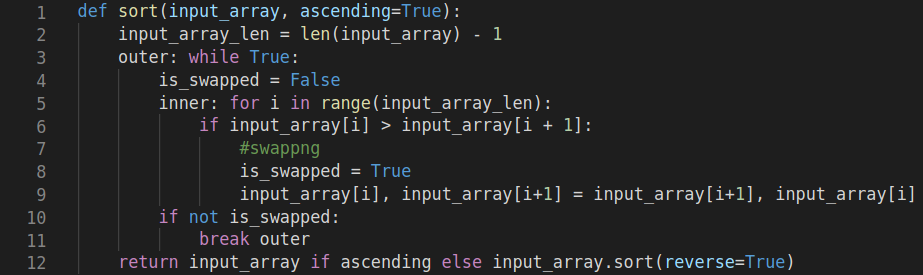
\includegraphics[width=\linewidth]{./9.png}
		\caption{کد برنامه}
	\end{center}
\end{figure}

\begin{itemize}
	\item \textbf{گراف \lr{ISP}}
	\begin{figure}[!h]
		\begin{center}
			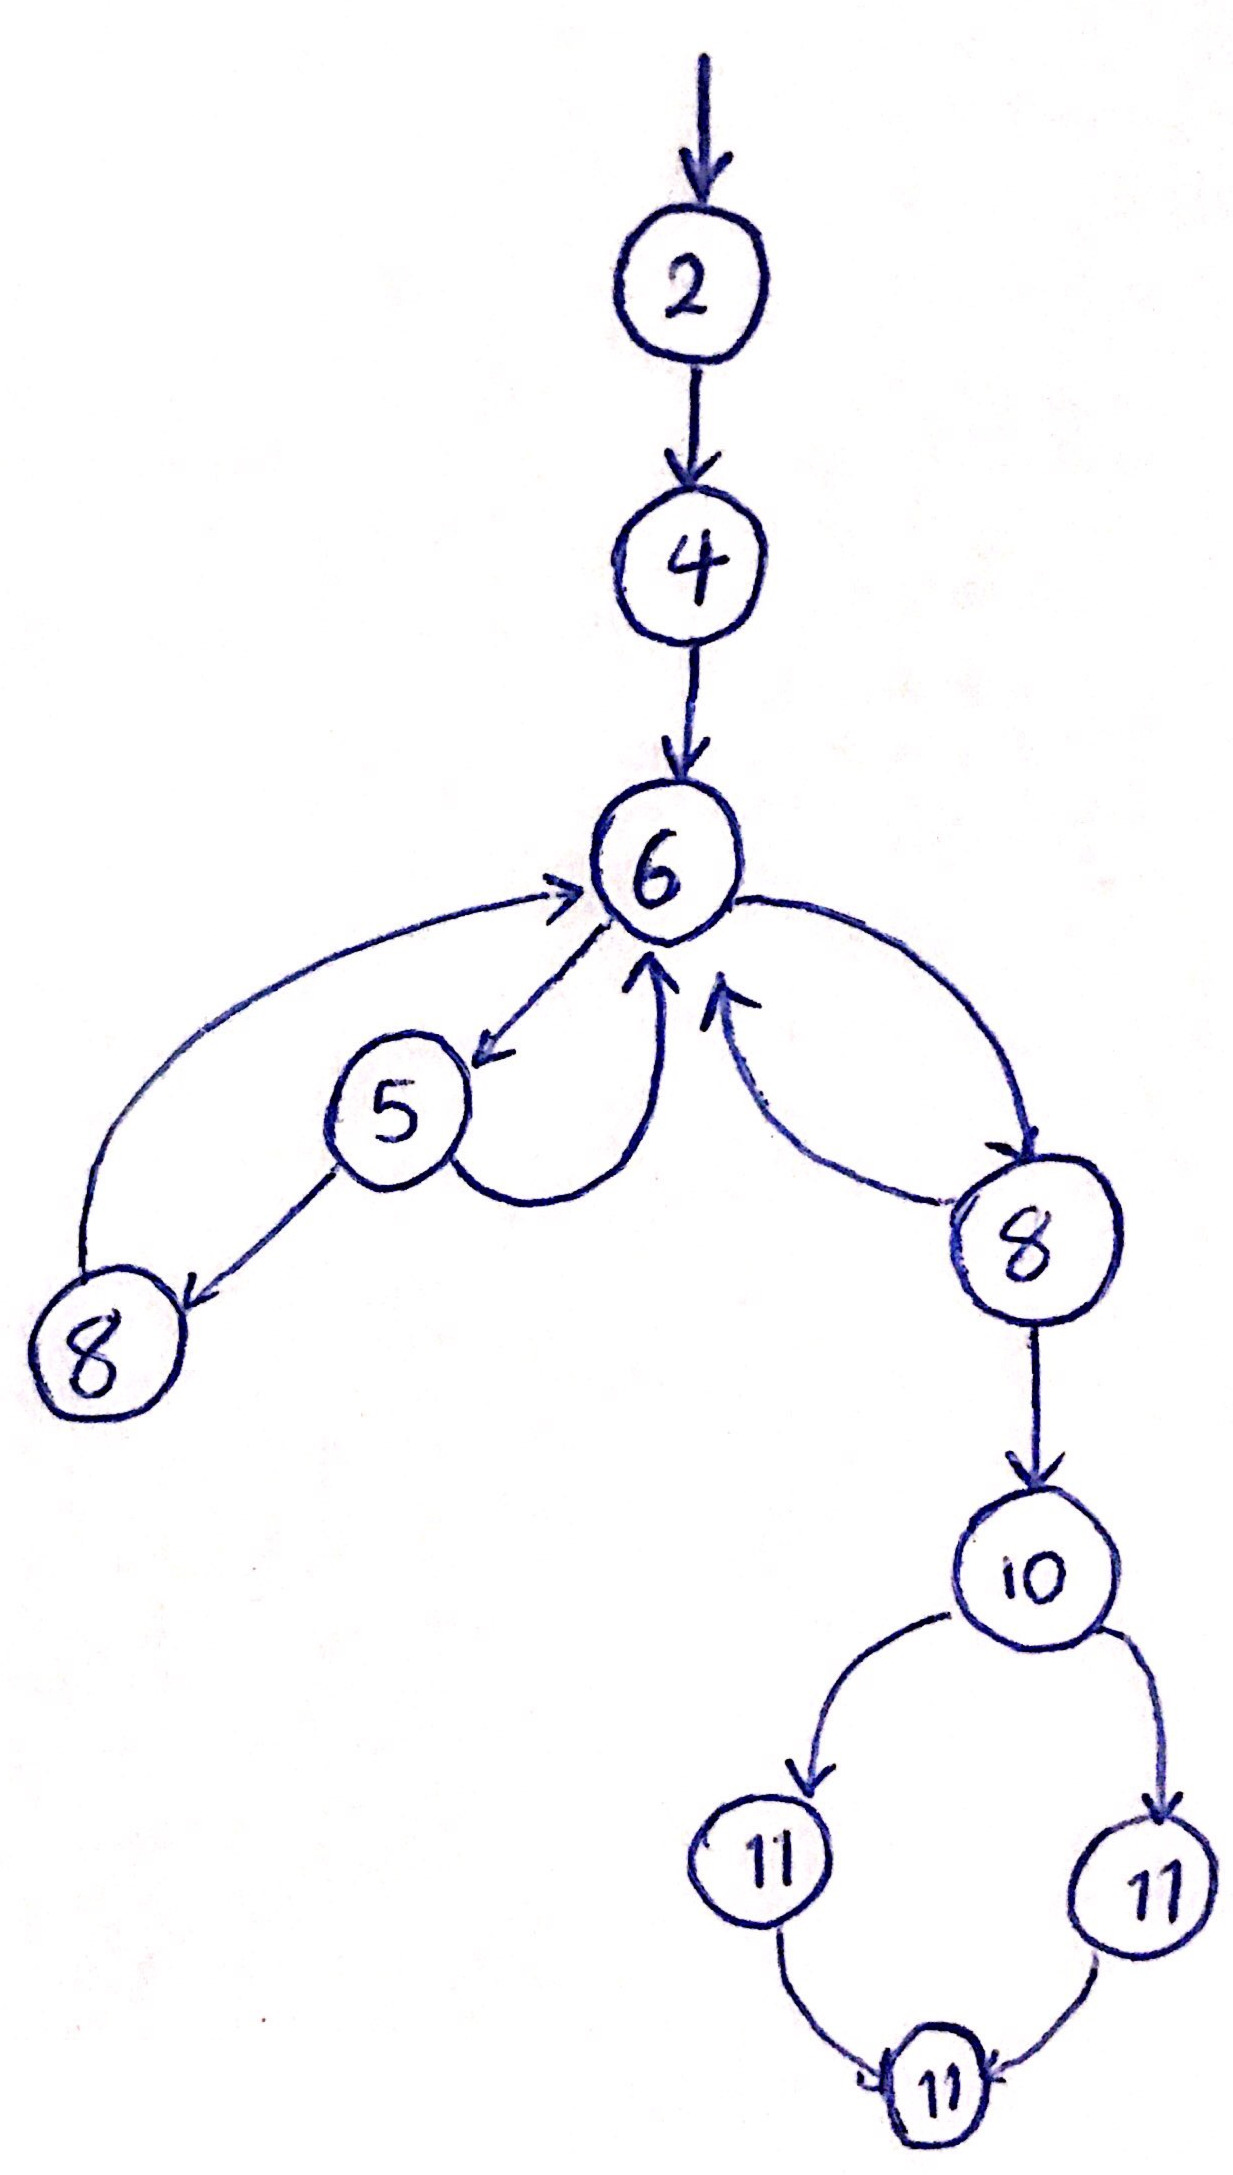
\includegraphics[scale=.5]{./9-2.jpg}
			\caption{گراف \lr{ISP} این گراف براساس شماره‌ی خط‌های کد ساخته شده است.}
		\end{center}
	\end{figure}
	\item \textbf{پوشش گره‌ها}\footnote{\lr{node coverage}}
	\begin{equation*}
	Node Coverage = \{[2, 4, 6, 5, 8, 8, 10, 11, 11], [2, 4, 6, 8, 10, 11, 11]\}
	\end{equation*}
	\item \textbf{بررسی راه و پوشش}
	
	به دلیل وجود حلقه امکان‌پذیر نیست.
	\item \textbf{پوشش یال‌ها\footnote{Edge Coverage}}
	\begin{equation*}
		Edge Coverage: {[2, 4, 6, 5, 8, 6, 8, 10, 11, 11], [2, 4, 6, 5, 6, 8, 6, 8, 10, 11, 11]}
	\end{equation*}
	
	\item 
	\lr{Predicate}
	شامل موارد زیر است:
	\begin{itemize}
		\item 
		\begin{equation*}
			input\_array[i] > input\_array[i + 1]
		\end{equation*}
		\item 
		\begin{equation*}
			is\_swapped
		\end{equation*}
		\item 
		\begin{equation*}
			ascending
		\end{equation*}
	\end{itemize}
	\item 
	عبارت‌ها \footnote{clauses}
	همان موارد قسمت قبل هستند که به آن‌ها مقدار \lr{True} و یا \lr{False} اختصاص گرفته است. بنابراین در کل ۸ حالت داریم. 
\end{itemize}